\documentclass{beamer}
\usepackage[utf8]{inputenc}
\usepackage[T1]{fontenc}
\usepackage{parskip}
\usepackage{graphicx}
\usepackage{subcaption}
\usepackage{amsmath}
\usepackage{pstricks-add, pst-node}

\usetheme{Berlin}

\title{Reconnaissance optique de musique : 
\newline Algorithme
\textit{stable path}}

\author{Wenhao LUO}
\date{\today}
\institute{Université de Quebec à Chicoutimi}

\AtBeginSection[]
{
    \begin{frame}
        \frametitle{Table of Contents}
        \tableofcontents[currentsection]
    \end{frame}
}
\begin{document}
\setbeamertemplate{footline}[frame number]

\begin{titlepage}
\end{titlepage}

\begin{frame}
    \frametitle{Table des matières}
    \tableofcontents
\end{frame}

\section{Introduction}
\begin{frame}
    \frametitle{Définition}
    Reconnaissance optique de musique, ou \textit{Optical Music Recognition} (OMR).
    \newline

    \begin{quotation}
        Optical Music Recognition is a field of research that investigates how to computationally read music
        notation in documents.
    \end{quotation}
\end{frame}

\begin{frame}
    \frametitle{Exemple}
    \begin{figure}
    \centering
    \begin{subfigure}{.5\textwidth}
        \centering
        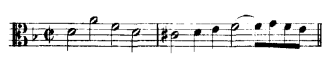
\includegraphics[width=.9\linewidth]{./img/music-notes.png}
        \caption{Un fragment d'une partition.}
    \end{subfigure}
    \begin{subfigure}{.5\textwidth}
        \centering
        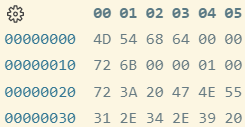
\includegraphics{./img/midi.png}
        \caption{Fichier \texttt{.mid} (MIDI) en hexa}
    \end{subfigure}
    \end{figure}
\end{frame}

\begin{frame}
    \frametitle{Pipeline}
    \begin{itemize}
        \item prétraitement d'image ;
        \item identification des notations musicales ;
        \item reconstruction des informations ;
        \item encodage et archivage.
    \end{itemize}
\end{frame}

\begin{frame}
    \frametitle{Identification des notations musicales}
    \begin{figure}
        \centering
        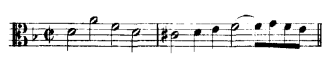
\includegraphics[width=0.7\linewidth]{img/music-notes.png}
    \end{figure}
    \begin{itemize}
        \item reconnaissance de \textit{staff} ;
        \item identification des symboles ;
        \item classification des symboles ;
        \item etc.
    \end{itemize}
\end{frame}

\section{Reconnaissance de \textit{staff}}
\subsection{Méthode auparavant}
\begin{frame}
    \frametitle{Projection horizontale}
    Identification du \textit{staff} par une projection.
    \begin{figure}
        \centering
        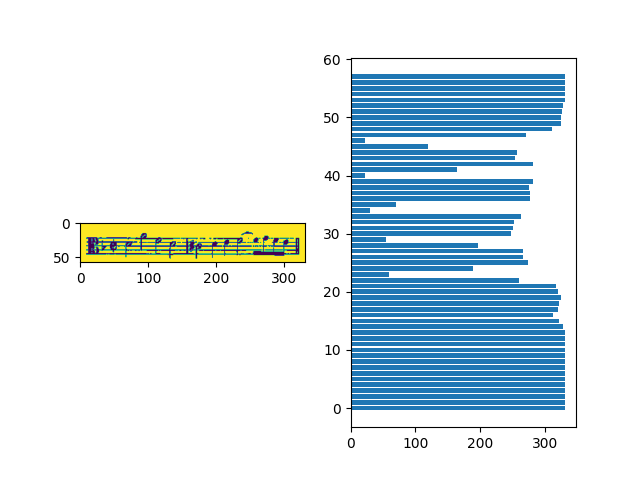
\includegraphics[width=0.8\linewidth, height=0.6\textheight]{img/project.png}
    \end{figure}
\end{frame}

\subsection{Méthode \textit{stable path}}
\begin{frame}
    \frametitle{Morphisme entre une image et un graphe}
    On définit un graphe à partir des pixels :
    \begin{figure}
    \begin{subfigure}{0.4\linewidth}
        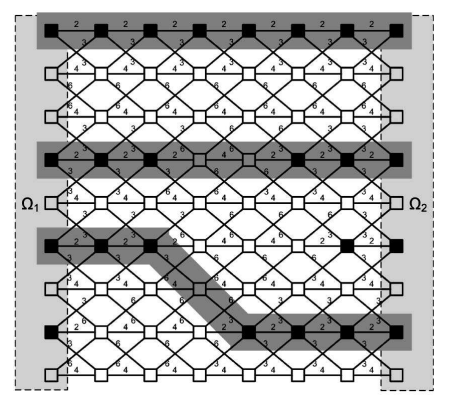
\includegraphics[height=0.5\textheight]{img/pixel-graph.png}
    \end{subfigure}
    \hspace*{\fill}
    \begin{subfigure}{0.4\linewidth}
        \begin{itemize}
            \item pixel noir : nœud ;
            \item connexion pixel-pixel : arête ;
            \item $(p_1, p_2, \cdots, p_n)$ : chemin.
        \end{itemize}
    \end{subfigure}
    \end{figure}
\end{frame}

\begin{frame}
    \frametitle{Définition de \textit{stable path}}
    \begin{quotation}
        A path $\mathcal{P}_{s, t}$ is a stable path between regions $\Omega_1$ and $\Omega_2$ if $\mathcal{P}_{s, t}$ is the shortest path between $s \in \Omega_1$ and the whole region $\Omega_2$, and $\mathcal{P}_{s, t}$ is the shortest path between $t \in \Omega_2$ and the whole region $\Omega_1$.
    \end{quotation}    
\end{frame}

\begin{frame}
    \frametitle{Retrouver les \textit{stable paths}}
    \dots qui sont les composantes du \textit{staff}.
    \begin{figure}
        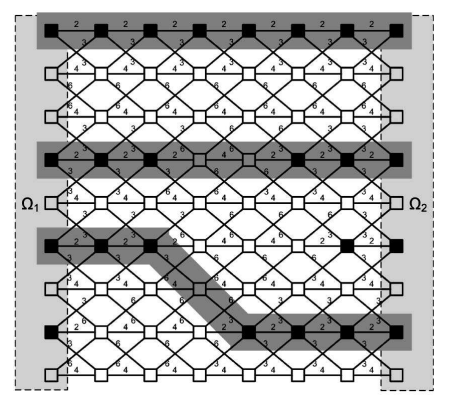
\includegraphics[height=0.5\textheight]{img/pixel-graph.png}
    \end{figure}
\end{frame}

\section{Conclusion}
\begin{frame}
    \frametitle{Conclusion}
    \begin{itemize}
        \item définition de OMR : reconnaissance optique de musique ;
        \item pipeline de cette recherche ;
        \item algorithme de reconnaissance de \textit{staff} :
        \begin{itemize}
            \item par projection, et
            \item par \textit{stable path}.
        \end{itemize}
    \end{itemize}
\end{frame}

\section*{Référence}
\begin{frame}
    \frametitle{Référence}
    \bibliography{ref.bib}
    \bibliographystyle{plain}
    \nocite{*}
\end{frame}

\end{document}